\documentclass[acmtog]{acmart}
\usepackage{graphicx}
\usepackage{subfigure}
\usepackage{natbib}

% Title portion
\title{Assignment 3 : Direct Lighting and Texturing} 
\author{Student Name: Zhanrui Zhang\\
        Student No. 2019533227\\
        Email: zhangzhr2@shanghaitech.edu.cn
}

% Document starts
\begin{document}
\maketitle

\vspace*{2 ex}


\section{Introduction}

In this assignment, we are required to render a scene by ray tracing with direct lighting. By generating rays through the direction of each pixel, the radiance is calculated. Then we convert the radiance of each pixel to the RGB value, and save the image.

\section{Implementation Details}
\subsection{Construct a Pin-hole Camera}
A pin-hole camera is defined by the following parameters.
\begin{enumerate}
    \item Film: film contanis the height and width of the image, as well as a pixel array which contains the radiance of each pixel.
    \item position: the world coordinate of the camera's position.
    \item forward: a vector defining the direction camera looking at.
    \item up: a vector defining the up direction of the camera, perpendicular to right and forward vector.
    \item right: a vector defining the right direction of the camera, perpendicular to up and forward vector.
    \item fov\_vertical: field of view in vertical direction. It defines how wide the camera could see.
    \item focal\_length: focal length defines how far the film plane is from the camera's position.
\end{enumerate}
To construct a pin-hole camera, first we need to specify the resolution of the film, the position in world coordinate, the focal lenght and the field of view.

Then the function `lookAt' is called to make further specification on camera. A coordinate `lookat' defines where the camera is looking at, together with the camera's position, the forward direction can be calculated. By another given vector `ref\_up', together with forward vector, right direction can be calculated by the cross product of forward and ref\_up. And the real up direction is just the cross product of right and forward vector.

\subsection{Generate Rays From Camera}
To generate a ray from the camera, two floating number `dx' and `dy' are given, specifying the ray's location on raster space. Then we need to calculate the coordinate in world space of this point.

First we normalize the raster space to $[0,1]\times[0,1]$, where $(0,0)$ locates in the left up corner, and $(1,1)$ locates in the right bottom corner. Then we transform the normalize device coordinate to $[-1,1]\times[-1,1]$. After that, we use the coordinate as the scaler, multiplying two basis vectors of the film to get the ray's position on film in world sapce.

The two basis vector are parallel to up and right direction respectively.
\[\vec{v}_{up} = \mathrm{focal\_len} \cdot \tan \frac{fov}{2}\]
\[\vec{v}_{right} = \mathrm{aspect\_ ratio} \cdot \mathrm{focal\_len} \cdot \tan \frac{fov}{2}\]

Once the ray's position on film by world coordinate is nailed down, the ray can be easily discribed by $\vec{O} + t\vec{D}$, where $\vec{O}$ is the camera's position, $\vec{D}$ is the the position of pixel minus the origin point of camera with normalization.

\subsection{Ray-Object Intersection}
In this assignment, we are required to implement ray-object interseciton method for spheres.

For a ray $\vec{O} + t\vec{D}$ and a sphere $x^2 + y^2 + z^2 = R^2$, we can calculate the intersection point by geometry method.
\begin{figure}[h]
    \centering
    \includegraphics[scale=0.25]{images/intersect.png}
\end{figure}
First we can calculate $|AE|$ by taking the dot product of $AC$ and $\vec{D}$, the we can calculate $|CE|^2$ by the Pythagorean theorem. When $|CE|^2 <0$ or $|CE|^2 < R^2$, the ray has no intersection with the object. Now $|BE| = |DE|$ can be calculated by $\sqrt{R^2 - |CE|^2}$.
$t_0 = |AE| - |BE|$, $t_1 = |AE| + |DE|$.

\subsection{Evaluate Radiance Based on Phong Model}
For rays hitting on the objcet, we can calculate the diffusion and specular based on Phong lighting model.

Diffusion is the light color times the surface color times the dot product of normal vector and the direction of in coming light.

Specular is the light color times the surface specular material times the dot product of viewing drection and reflection direction to the power of shineness.

\subsection{Ray Tracing with Direct Lighting}
For each pixel, we generate a ray through the center of pixel. If the pixel has no intersection with any object in the scene, we assume that no light is coming from this direction, and the radiance of this pixel will be set to zero. If the ray first intersects with the light, then the radiance of the pixel is just the light coming from the light. We just set the radiance to the color of the light.

When the ray first intersects with an object, we need to create a new ray from the intersection point to the light. If the new ray intersects with some geometry first, it means that the light source is invisible for that point, so we just return the value of ambient light. Otherwise, we calculate the radiance of the reflection light based on Phong lighting model. For area light, we need to create a series of sampling point on the light, treating each sampling point as a point light. Then we add radiance for all sampling point together, and divide by the number of sampling point (because the radiance of a pixel should not be relavent to the number of sampling point).

\subsection{Anti-aliasing}
To enable anti-aliasing, we need to sample more than one ray in each pixel. The easy way to do this is to take sample point with uniform grid and take the average value as the radiance of the pixel.
To better demostrate the result, an new object `Ground', which is a infinite plane with checkerd box texture. The results are shown in pictures bellow.

\begin{figure}[h]
    \centering
    \subfigure[Without Anti-aliasing]
    {
        \begin{minipage}[b]{.4\linewidth}
            \centering
            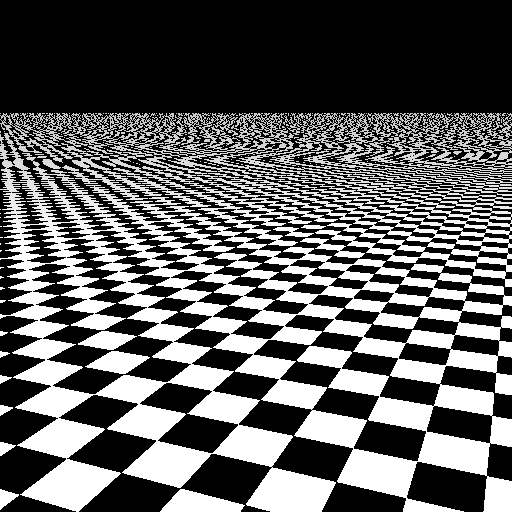
\includegraphics[scale=0.4]{images/ground_gird_spp1.png}
        \end{minipage}
    }
    \subfigure[SPP=4, uniform gird]
    {
        \begin{minipage}[b]{.4\linewidth}
            \centering
            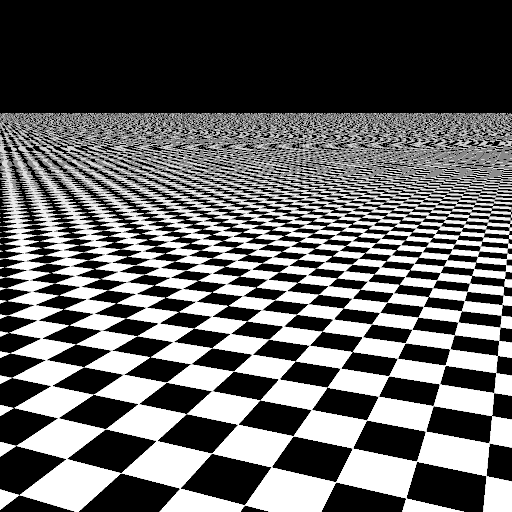
\includegraphics[scale=0.4]{images/ground_gird_spp4.png}
        \end{minipage}
    }
    \\
    \subfigure[SPP=4, random sampling] 
    {
        \begin{minipage}[b]{.4\linewidth}
            \centering
            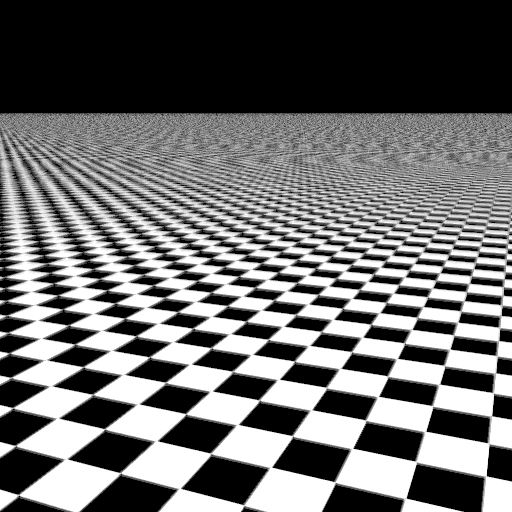
\includegraphics[scale=0.4]{images/ground_random_spp4.png}
        \end{minipage}
    }
    \subfigure[SPP=576, uniform grid]
    {
        \begin{minipage}[b]{.4\linewidth}
            \centering
            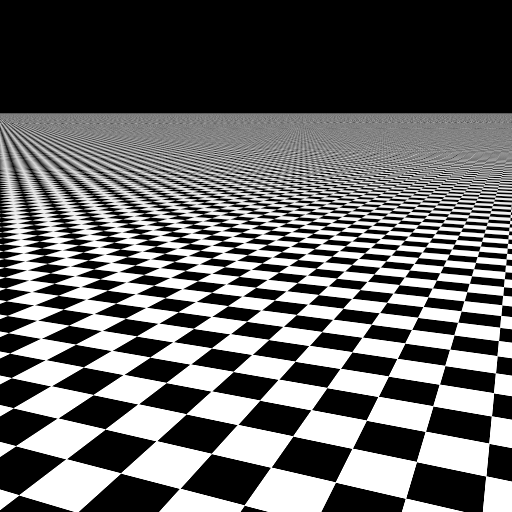
\includegraphics[scale=0.4]{images/ground_grid_spp576.png}
        \end{minipage}
    }
    \caption{Result of Anti-aliasing}
\end{figure}
    
As the SPP(sample per pixel) increase, the aliasing effect becomes less significant. However, the rendering time also increases. Take random sample rather than sampling uniform grid can improve the result greatly, leading to a result similar to much higher SPP in uniform gird.
    
\subsection{Cube Map for Environment Mapping}
First we need to create a cube. A new geometry `Box' is added, which contains 6 textures for 6 faces for the cube. Meanwhile a new light class named `EnvironmentLight' is added. For rays intersecting with the camera, we calculate its intersection distance for all 6 faces. Take the least positive distance as the intersection point. Once we know which face the ray is intersecting with, we can know the 2-D local coordinate on that face, thus the uv coordinate on texture can be easily figured out. And we just return the corresponding color value.
    
For geometry in the scene, we just calculate the perfect specular ray and get the environment light of evaluate by the reflection ray.
    
\subsection{Mipmap}
First we need to generate a seires of Texture with different resolution. So we need to shrink the original texture. For simplicity, we just perform a bilinear interpolation recusively, until the new texture has only 1 pixel left.
    
The most important part for mipmap is to determine which layer to evaluate from. The goal is to make the pixel size on texture match the pixel size on screen. So we can calculate the size a pixel can cover on objcet and the size one texture pixel cover and calculate the ratio.
    
First we need to calculate how long can the width of a screen pixel cover after being casted to the surface of an object. It can be done with some simple geometry.
    
\begin{figure}[h]
    \centering
    \includegraphics[scale=0.4]{images/geo.png}
\end{figure}

Suppose $HE$ is the width of the pixel, $IF$ is its range on surface of object. The light is $\vec{O} + t\vec{D}$
\[\frac{HE}{AE} = \frac{GF}{AF}\]
\[L = IF = \frac{2 t \cdot \tan \frac{\mathrm{fov}}{2}}{- r \vec{N}\cdot \vec{D}}\]

Where t is the distance to the intersection point and r is the vertical resolution of the raster.

Then we need to calculate how long the width of a pixel on texture can cover after it is mapped on to the surface of the object. This depends on how the texture is wrapped on the surface of the
object. More specifically, it depends on the way of uv mapping and the texture's resolution.
As to the scaling caused by the uv mapping, we can obtain the scaling factor by calculate the determinant of Jacobian matrix of coordinate transformation. We need to specifically calculate this factor for each different object.

Let $T$ be the transformation mapping $(u,v)$ to $(x,y,z)$, 
\[
    J_T = \left(\begin{matrix}
        \frac{\partial x}{\partial u} & \frac{\partial x}{\partial v}\\
        \frac{\partial y}{\partial u} & \frac{\partial y}{\partial v}\\
        \frac{\partial z}{\partial u} & \frac{\partial z}{\partial v}
    \end{matrix}\right)
\]
$|J_T|$ defines how long the unit length in uv space is stretched to when mapped into world space. 

Let $m$ be the resolution of texture. The texture pixel's real world width is $W = \frac{|J_T|}{m}$.
So the proportion between a screen pixel and texture pixel on the surface of object is $\frac{L}{W}$. And the level we should take in mipmap is $\log\frac{L}{W}$. In practice, we need to take two closest layers to $\log\frac{L}{W}$ and interpolate them together.
\begin{figure}[h]
    \centering
    \subfigure[Without Mipmap]
    {
        \begin{minipage}[b]{.4\linewidth}
            \centering
            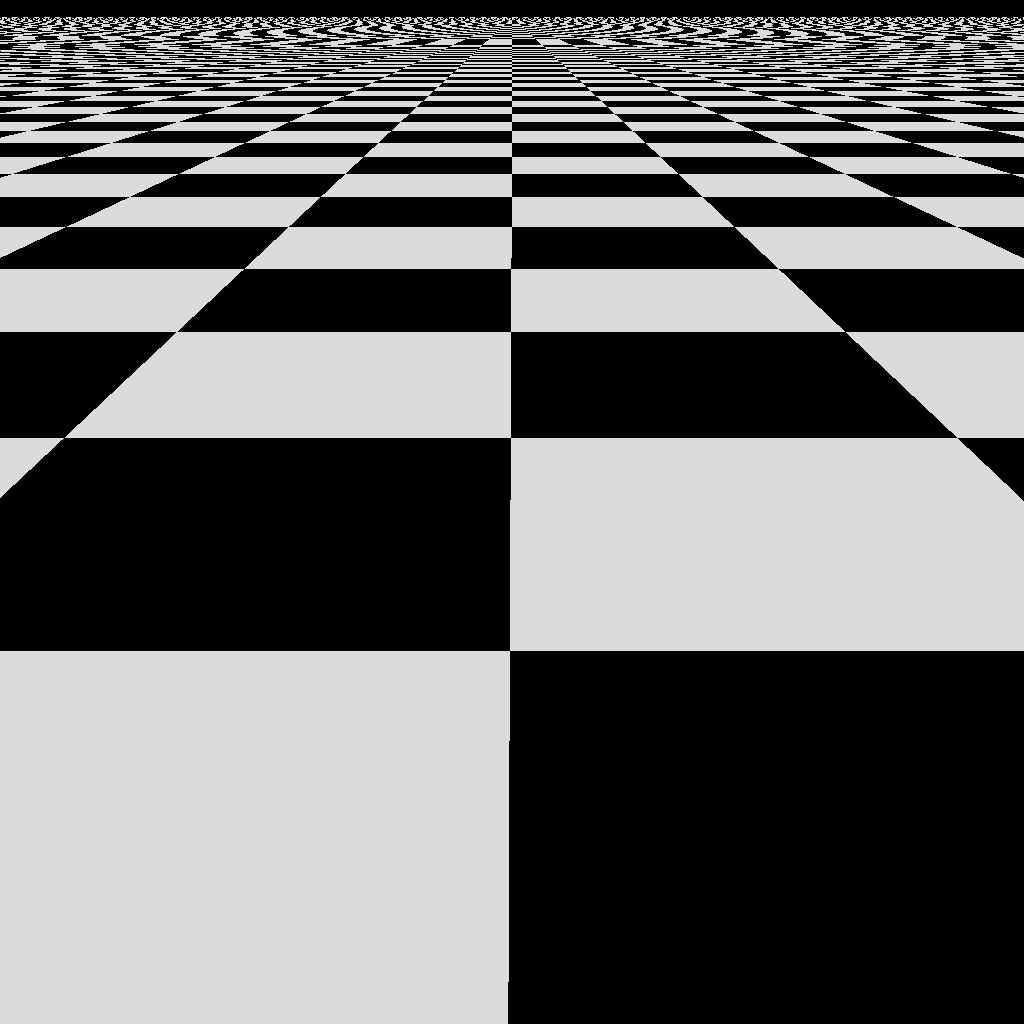
\includegraphics[scale=0.22]{images/no_mipmap.png}
        \end{minipage}
    }
    \subfigure[With Mipmap]
    {
        \begin{minipage}[b]{.4\linewidth}
            \centering
            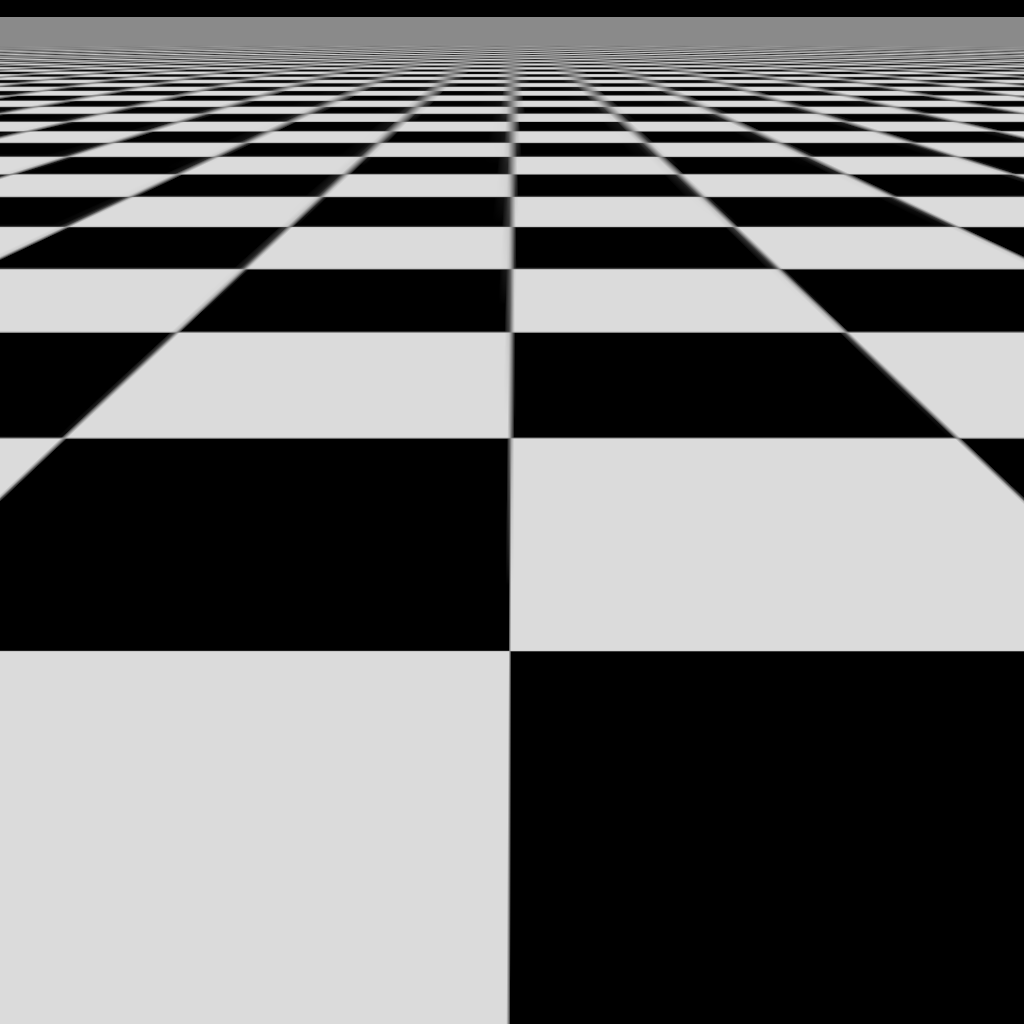
\includegraphics[scale=0.22]{images/mipmapped.png}
        \end{minipage}
    }
    \caption{Mipmap}
\end{figure}

As can be shown, there are actually some overblur problem. This is beacuse that the checkerd box texture is not friendly to bilinear interpolation when creating texture with different resolution. Intermediate levels of texture are not properly blurred as expected since the edges of each box happen not to be interpolated. A better approach may be cubic spline interpolaion, but it is not implemented due to limited time.

\section{Results}
The rendering result is given as follow. Each picture is rendered with 256 sampling points on the light, and 256 sampling point per pixel.

\begin{figure}[h]
    \centering
    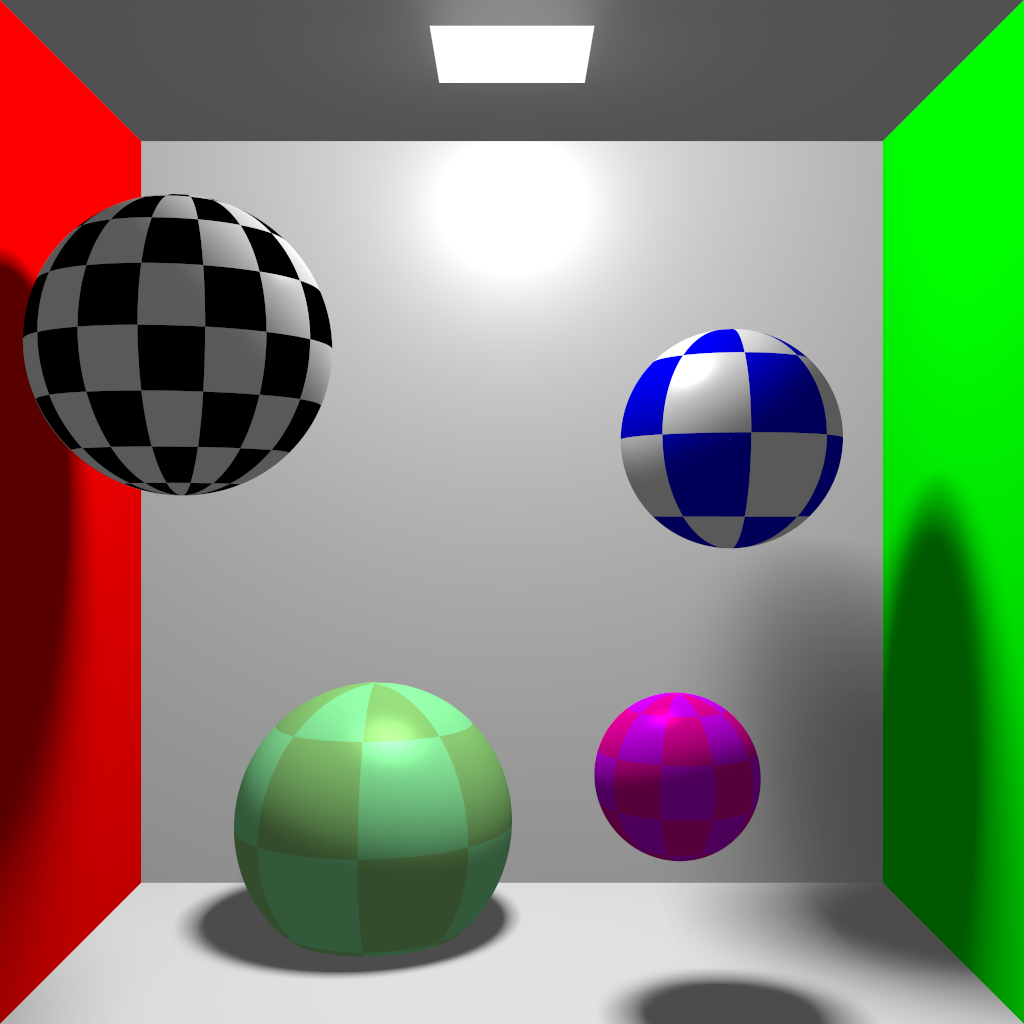
\includegraphics[scale=0.2]{images/output_spp1024_set1.png}
    \caption{Set1}
\end{figure}

\begin{figure}[h]
    \centering
    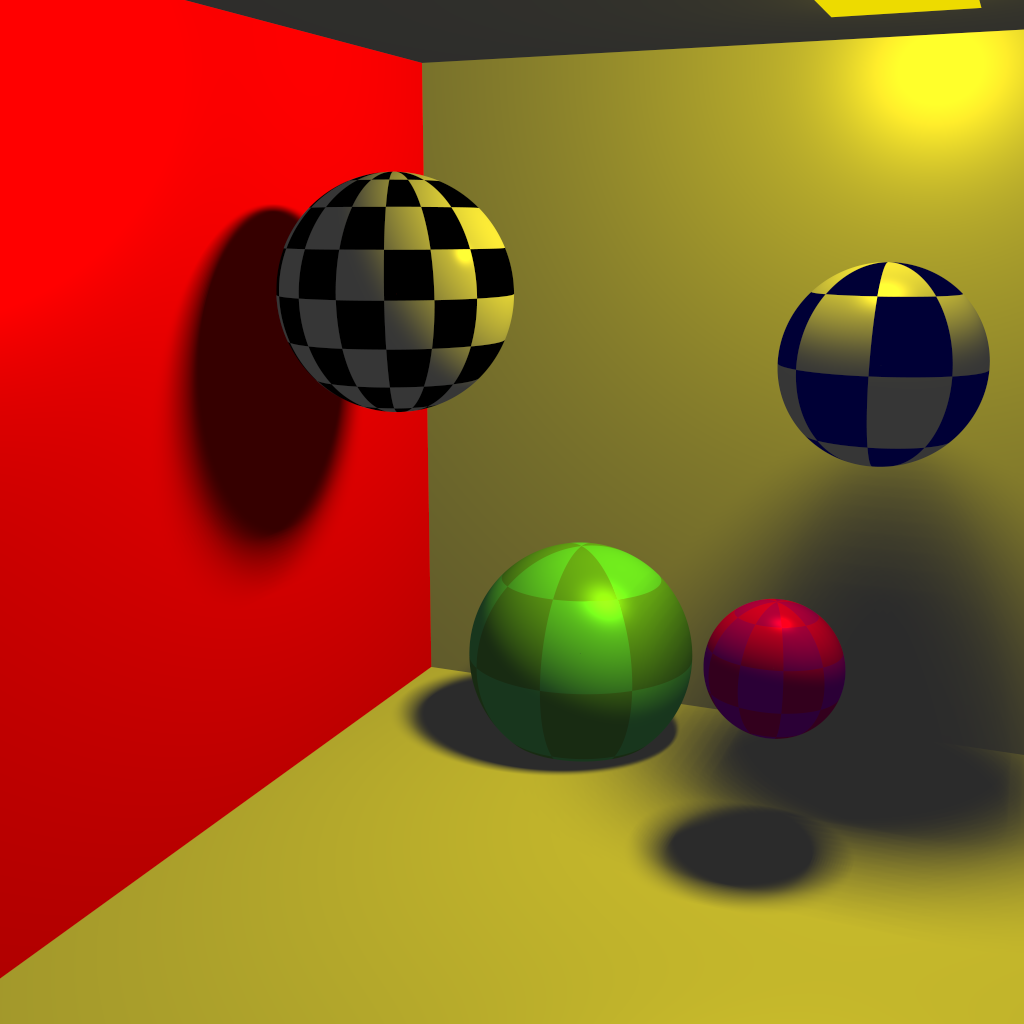
\includegraphics[scale=0.2]{images/output_set2_spp256.png}
    \caption{Set2}
\end{figure}

\begin{figure}[h]
    \centering
    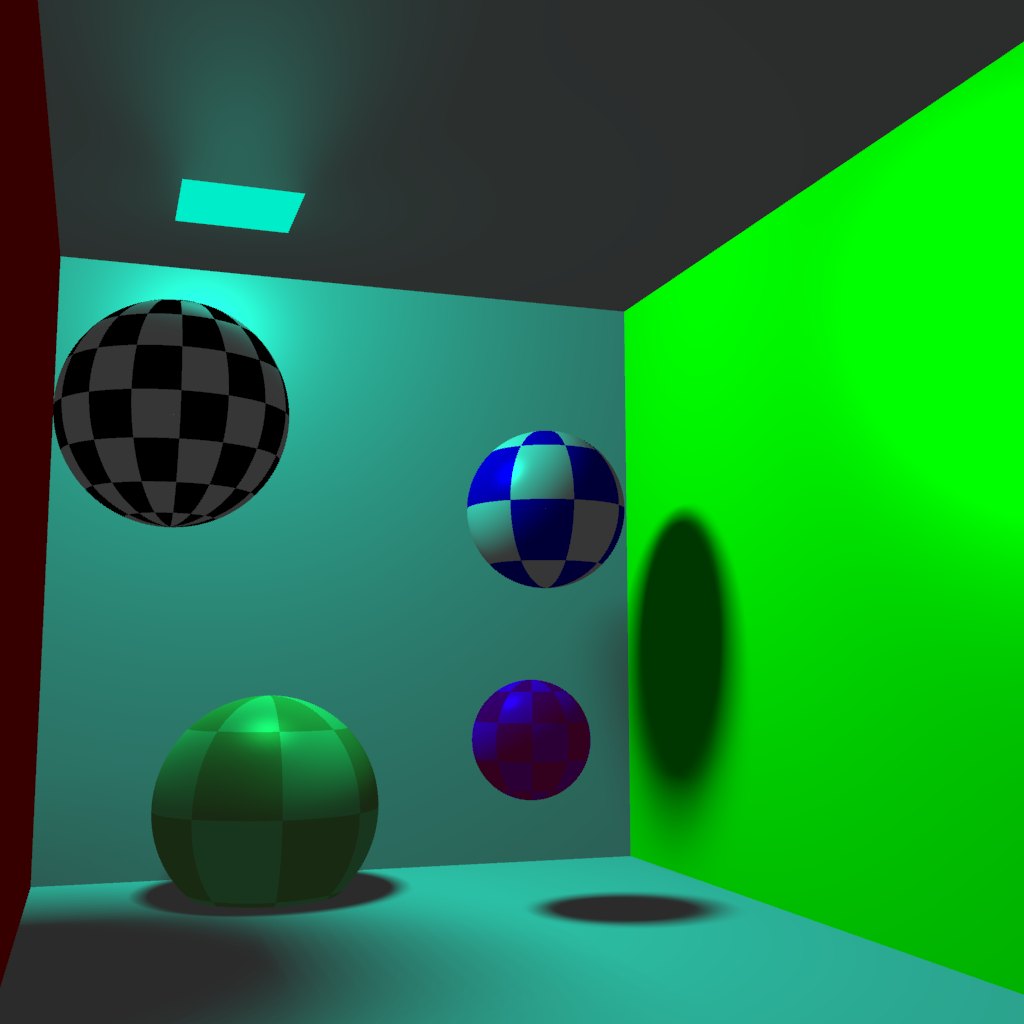
\includegraphics[scale=0.2]{images/output_set3_spp256.png}
    \caption{Set3}
\end{figure}

\begin{figure}[h]
    \centering
    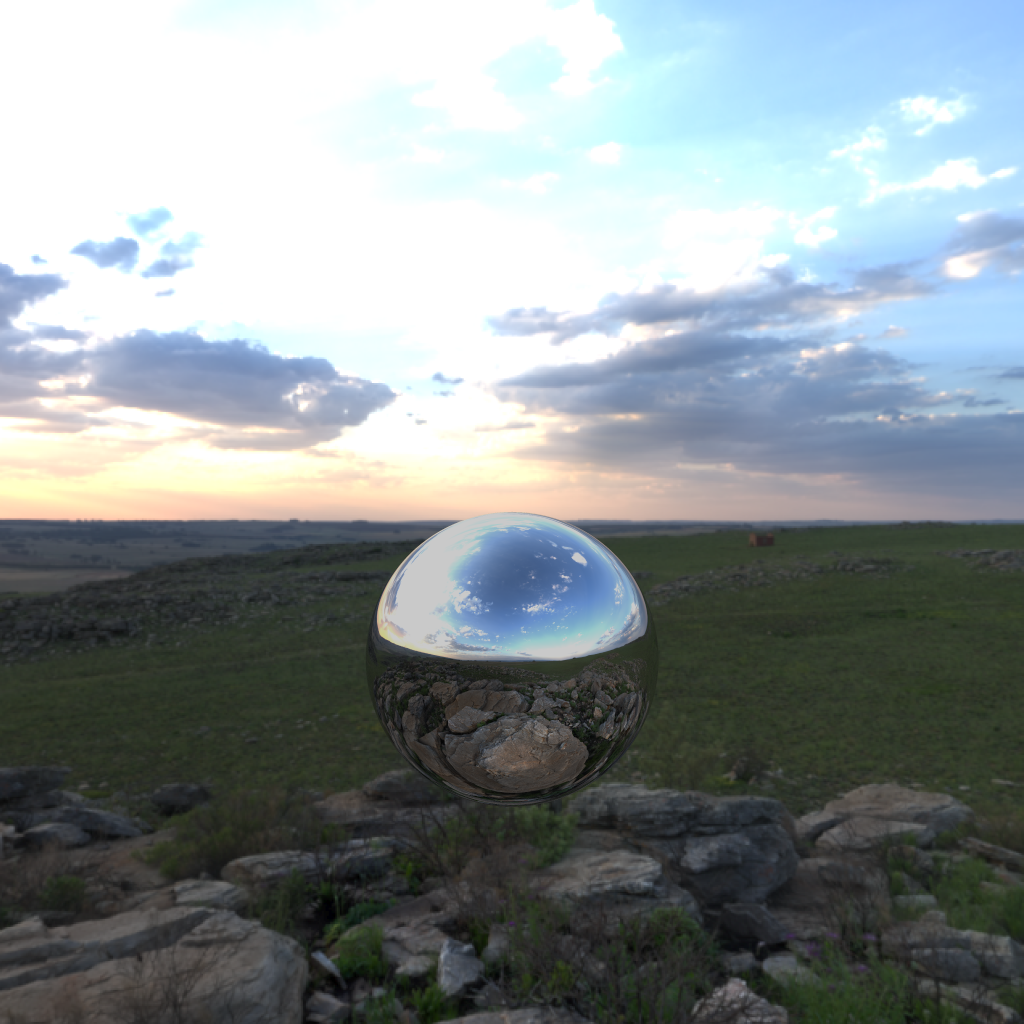
\includegraphics[scale=0.2]{images/environment_light.png}
    \caption{Environment Lighting}
\end{figure}

\end{document}
